\chapter{Переходный процесс в неподвижных магнитосвязанных цепях}
\label{chap:4 perehodnyi_protcess_v_nepodvizhnykh_magnitosviazannykh_tcepiakh}

\section{Общие замечания}
\label{sec:4-1}

Протекание электромагнитного переходного процесса в магнитносвязанных цепях имеет некоторые характерные особенности. Рекомендуется обратить особое внимание на основные закономерности и соотношения, рассматриваемые в настоящей главе; они в значительной мере облегчат понимание более сложных явлений, которые исследуются в дальнейшем применительно к вращающимся электрическим машинам.

В качестве основной предпосылки в соответствии с ранее принятыми допущениями считаем, что между токами и напряжениями рассматриваемых цепей сохраняется линейная зависимость и, следовательно, они могут быть связаны линейными дифференциальными уравнениями с постоянными коэффициентами. Для силовых трансформаторов и автотрансформаторов в условиях короткого замыкания (или значительных перегрузок) это допущение практически выполняется, поскольку основные магнитные потоки и обусловленное ими насыщение магнитопроводов при этом становится меньше.

Иное положение имеет место в измерительных трансформаторах тока при протекании по их первичным обмоткам больших токов короткого замыкания (или перегрузки). Здесь ток во вторичной обмотке сильно зависит от насыщения магнитопровода. Последний вопрос представляет предмет специального исследования.

Указанное допущение также не пригодно, когда рассматривается переходный процесс при включении
силовых трансформаторов и автотрансформаторов и при внезапном сбросе их нагрузки. Правильное представление о протекании такого переходного процесса можно получить только при учете изменения насыщения их магнитопроводов (\colorbox{red}{см. § 4-6}).

Характер изменения свободных токов, как известно, определяется параметрами элементов рассматриваемой схемы и соотношениями между ними. Поэтому полученные ниже закономерности изменения свободных токов справедливы при любых э.~д.~с. источников питания.

От величины э.~д.~с., естественно, зависят начальные значения свободных токов.

\section{Основные уравнения и соотношения}
\label{sec:4-2}

Рассмотрим переходный процесс при включении на некоторое напряжение $ u(t) $ контура с $ L_1 $ и $ r_1 $ связанного взаимной индуктивностью $ M $ с другим контуром, индуктивность и активное сопротивление которого $ L_2 $ и $ r_2 $. По существу это является процессом включения воздушного трансформатора с закороченной вторичной обмоткой (рис. 4-1). Условимся, что все параметры и величины второго контура приведены к стороне первого контура.

\begin{floatingfigure}[lflt]{0.45\linewidth}
	\centering
	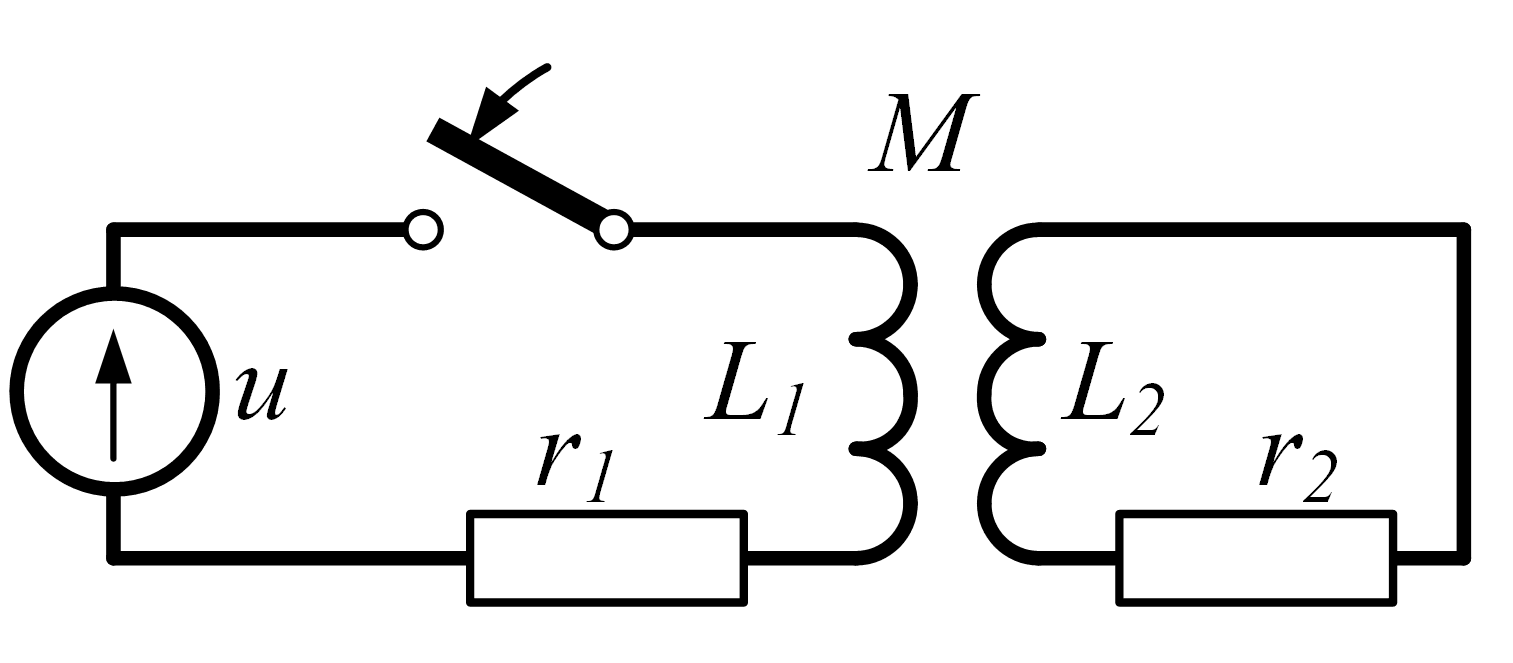
\includegraphics[width=0.40\linewidth]{pic/4-1}
	\caption{Простейшая цепь с магнитной связью.}
	\label{ris:4-1 simplest_circut}
\end{floatingfigure}

Для каждого контура соответственно имеем:

постоянные времени

$$ T_{10} = \frac{L_1}{r_1}\text{~сек.} $$

и

$$ T_{20} = \frac{L_2}{r_2}\text{~сек.}$$

(индекс 0 у постоянной времени указывает, что она определена при всех разомкнутых контурах, с которыми данный контур имеет магнитную связь);

коэффициенты рассеяния

$$ \sigma_1 = \frac{L_1 - M}{L_1} $$

и

$$ \sigma_2 = \frac{L_2 - M}{L_1}\text{~.} $$

Коэффициент магнитной связи между контурами

$$ k = \frac{|M|}{\sqrt{L_1 L_2}} $$

и общий коэффициент рассеяния

\begin{equation}
	\sigma = 1 - k^2 = 1 - \frac{M^2}{L_1 L_2} = \sigma_1 + \sigma_2 - \sigma_1 \sigma_2\text{;}
	\label{eq:4-1 sigma}
\end{equation}

при малых значениях $ \sigma_1 $ и $ \sigma_2 $ можно принимать

\begin{equation}
    \sigma \approx \sigma_1 + \sigma_2
	\label{eq:4-2 sigma}
\end{equation}

Считая, что при принятых положительных направлениях токов магнитные потоки самоиндукции и взаимной индукции в каждой катушке совпадают, имеем:

\begin{equation}
    \left.\begin{matrix}
        u(t) = i_1 r_1 + L_1 \frac{di_1}{dt} + M \frac{di_2}{dt}\text{;}\\ 
        0 = i_2 r_2 + L_2 \frac{di_2}{dt} + M \frac{di_1}{dt}
    \end{matrix}\right\}
	\label{eq:4-3 diffur}
\end{equation}

в операторной форме (при нулевых начальных условиях)

\begin{equation}
    \left.\begin{matrix}
        u(p) = r_1 I_1(p) + L_1 p I_1(p) + M p I_2(p) \text{;}\\ 
        0 = r_2 I_2(p) + L_2 p I_2(p) + M p I_1(p) \text{.}
    \end{matrix}\right\}
	\label{eq:4-4 diffur}
\end{equation}

Решение системы (\ref{eq:4-4 diffur}) легко получить простой подстановкой. Из второго уравнения имеем:

\begin{equation}
    I_2(p) = - \frac{M p}{r_2 + L_2 p} I_1 \text{;}
	\label{eq:4-5 I_2}
\end{equation}

после подстановки (\ref{eq:4-5 I_2}) в первое уравнение (\ref{eq:4-4 diffur}) найдем:

\begin{equation}
    I_1(p) = \frac{u(p)}{z_1(p)} \text{,}
	\label{eq:4-6 I_1}
\end{equation}

где

\begin{equation*}
    z_1(p) = r_1 + (L_1 - \frac{M^2 p}{r_2 + L_2 p}) p = r_1 + \frac{1 + \sigma T_{20} p}{1+T_{20} p} L_1 p =
\end{equation*}

\begin{equation}
    = \frac{\sigma T_{10} T_{20} p^2 + (T_{10} + T_{20}) p + 1}{(1 + T_{20} p)} r_1
	\label{eq:4-7 z_1}
\end{equation}

— операторное сопротивление первого контура с учетом магнитносвязанного с ним короткозамкнутого второго контура.

Из (\ref{eq:4-7 z_1}) следует, что влияние короткозамкнутого контура сказывается в снижении $ L_1 $, причем оно тем сильнее, чем меньше рассеяние и больше постоянная времени $ T_{20} $. Напротив, в пределе, когда $ \sigma = 1 $, т.~е. при отсутствии магнитной связи, индуктивность $ L_1 $ неизменна.

Из характеристического уравнения $ z_1(p) = 0 $ находим его корни:

\begin{equation*}
    \label{eq:4-8 p_1,2}
    p_{1,2} = \frac{-(T_{10}+T_{20}) \pm \sqrt{(T_{10}+T_{20})^2-4\sigma T_{10}T_{20}}}{2 \sigma T_{10}T_{20}}=
\end{equation*}

\begin{equation}
    =-\frac{(T_{10}+T_{20})}{2 \sigma T_{10}T_{20}} \times (1 \mp q) \text{,}
\end{equation}

где

\begin{equation}
    \label{eq:4-9 q}
    q=\sqrt{1-\frac{4\sigma T_{10}T_{20}}{(T_{10}+T_{20})^2}}\text{.}
\end{equation}

Поскольку всегда $ (T_{10}+T_{20})^2 > 4\sigma T_{10}T_{20} $, оба корня являются действительными, меньшими нуля.

Следовательно, свободный ток каждого контура представляет собой сумму двух свободных токов, один из которых затухает по экспоненте с постоянной времени\footnote{Индексация постоянных времени умышленно принята отличной от обозначения рассматриваемых контуров, чтобы исключить ошибочное представление, что каждая из этих постоянных времени характеризуется параметрами якобы только одного из данных контуров.}

\begin{equation}
    \label{eq:4-10 T}
    T'=-\frac{1}{p}=\frac{2}{(1-q)}\frac{\sigma T_{10}T_{20}}{(T_{10}+T_{20})}=\frac{1+q}{2}(T_{10}+T_{20})\text{,}
\end{equation}

а другой — с постоянной времени

\begin{equation}
    \label{eq:4-11 T''}
    T''=-\frac{1}{p_2}=\frac{2}{(1+q)}\frac{\sigma T_{10}T_{20}}{(T_{10}+T_{20})}=\frac{1-q}{2}(T_{10}+T_{20})\text{,}
\end{equation}

отношение между которыми

\begin{equation}
    \label{eq:4-12 T'T''}
    \frac{T'}{T''}=\frac{1+q}{1-q}\text{.}
\end{equation}

Как видно, $ T' $ всегда больше $ T'' $, причем различие между ними возрастает с уменьшением рассеяния. В пределе при $ \sigma = 0 $ имеем: $ T' = T_{10} + T_{20} $ и $ T'' = 0 $.

При включении контура на постоянное напряжение $ U \Doteq U(p) = U/p $ для изображения тока первого контура имеем:

\begin{equation*}
    I_1(p)=\frac{U}{pz_1(p)}
\end{equation*}

Используя известную формулу разложения (или ее видоизменение, так называемую формулу включения) и произведя ряд преобразований, получим временную функцию тока этого контура:

\begin{equation}
    \label{eq:4-13 i_1}
    i_1(t)=i_1+i'_1+i''_1=\frac{U}{r_1}-\frac{U(T_{10}-T'')}{r_1(T'-T'')}e^{-t/T'}-\frac{U(T_{10}-T'')}{r_1(T'-T'')}e^{-t/T''}\text{,}
\end{equation}

где

$ i_1 $ - принужденный или установившийся ток;

$ i'_1 $ - медленно затухающий свободный ток;

$ i''_1 $ - быстро затухающий свободный ток.

Соотношение между начальными значениями этих свободных токов определяется постоянными времени:

\begin{equation}
    \label{eq:4-14 i_i}
    \frac{i''_{1|0|}}{i'_{1|0|}}=\frac{T_{20}-T''}{T_{10}-T''}\text{.}
\end{equation}

Аналогично находим выражение для тока во втором контуре:

\begin{equation}
    \label{eq:4-15 i_2}
    i_2(t)=i'_2+i''_2=-\frac{MU}{L_1L_2}\frac{T_{10}T_{20}}{(T'-T'')}(e^{-t/T'}-e^{-t/T''})\text{,}
\end{equation}

из которого видно, что при включении контура на постоянное напряжение принужденный ток во втором контуре, естественно, отсутствует, а начальные значения свободных токов равны и взаимно противоположны:

\begin{equation}
    \label{eq:4-16 i''}
    i''_{2|0|}=-i'_{2|0|}\text{.}
\end{equation}

Их связь с одноименными свободными токами первого контура выражается соотношениями:

\begin{equation}
    \label{eq:4-17 i'2}
    i'_2=\frac{M}{L_2}\frac{T_{20}}{(T_{10}-T'')}i'_1\text{;}
\end{equation}

\begin{equation}
    \label{eq:4-18 i''2}
    i''_2=-\frac{M}{L_2}\frac{T_{20}}{(T_{20}-T'')}i''_1\text{.}
\end{equation}

Для рассматриваемого переходного процесса на \colorbox{red}{рис. 4-2,а} приведены кривые изменения токов и их отдельных слагающих, причем откладываемое по оси абсцисс время выражено в долях от $ Т_{10} $. Ток $ i_1(t) $ стремится к своему принужденному значению, а ток $ i_2(t) $ сначала возрастает до своего максимума, а затем затухает, стремясь к нулю. Момент наступления максимума легко найти из уравнения $ di_2 / dt = 0 $:

\begin{equation}
    \label{eq:4-19 t_m}
    t_m=\frac{T'T''}{T'-T''}~ln\frac{T'}{T''}\text{.}
\end{equation}

Подставив (\ref{eq:4-19 t_m}) в (\ref{eq:4-15 i_2}), получим:

\begin{equation}
    \label{eq:4-20 i2}
    i_{2m}=-\frac{MU}{L_1L_2}\frac{T_{10}T_{20}}{(T'-T'')}(e^{-t_m/T'}-e^{-t_m/T''})\text{.}
\end{equation}

Для сопоставления на \colorbox{red}{рис. 4-2,6} показаны кривые изменения токов при закорачивании первого контура, после того как в нем наступил установившийся режим. В этом случае все величины свободных токов остаются такими же, как и при рассмотренном выше процессе включения, но их знаки меняются на обратные При этом, разумеется, принужденные токи в обоих контурах отсутствуют.

По характеру кривых изменения токов $ i_1 $ и $ i_2 $ (\colorbox{red}{рис 4-2}) видно, что в начальной стадии переходного процесса изменение токов обусловливается главным образом быстро затухающими свободными токами, а в последующей практически только медленно затухающими свободными токами. Ток намагничивания, определяемый суммой токов ($ i_1 + i_2 $), практически изменяется экспоненциально с постоянной времени $ T' $ так как сумма быстро затухающих токов $ (i_1''+i_2') $ очень мала. Последняя равна нулю при $ \sigma = 0 $.

Медленно затухающие свободные токи практически связаны с изменением только общего магнитного потока или потока взаимоиндукции между контурами, а быстро затухающие — c изменением только потоков рассеяния контуров.

Таким образом, магнитная связь между контурами вначале убыстряет переходный процесс, а затем, напротив, замедляет его. При постоянном коэффициенте рассеяния $ \sigma $ это проявляется тем интенсивнее, чем больше постоянная времени влияющего контура ($ T_{20} $). Это хорошо видно на \colorbox{red}{рис 4-3}, где приведены для нескольких значении $ T_{20} $ кривые изменения токов $ i_1 $ и $ i_2 $. Кривые при $ T_{20} = 0 $ соответствуют условию, при котором влияющий контур отсутствует (или разомкнут); соответственно при $ T_{20}=\infty $ — когда он является сверхпроводящим. В последнем случае наведенный свободный ток $ i_2 $ стремится к своему наибольшему значению, а затем остается неизменным, поскольку потерь в этом контуре нет.

\section{Влияние рассеяния}
\label{sec:4-3}

Выясним теперь, как влияет рассеяние на соотношения между постоянными времени затухания свободных токов, а также между начальными значениями этих токов. Для этого установим вначале дополнительные соотношения, которые вытекают из известных свойств корней квадратного уравнения\footnote{Корни уравнения $ ax^2 + bx + c = 0 $ связаны между собой соответствиями: $ x_1 + x_2 = -\frac{b}{a} $ и $ x_1 x_2 = \frac{c}{a} $.}. Из них имеем:

\begin{equation}
    \label{eq:4-21 p1p2}
    p_1+p_2=-(\frac{1}{T'}+\frac{1}{T''})=-\frac{T_{10}+T_{20}}{\sigma T_{10}T_{20}}\text{,}
\end{equation}

или

\begin{equation*}
    \frac{T'+T''}{T'T''}=\frac{T_{10}+T_{20}}{\sigma T_{10}T_{20}}\text{;}
\end{equation*}

помимо того,

\begin{equation*}
    p_1p_2=\frac{1}{T'T''}=\frac{1}{\sigma T_{10}T_{20}}\text{,}
\end{equation*}

т.~е.

\begin{equation}
    \label{eq:4-21a TT}
    T'T''=\sigma T_{10}T_{20}
    \tag{\ref*{eq:4-21 p1p2}а}
\end{equation}

или 

\begin{equation}
    \label{eq:4-21b sigma}
    \sigma = \frac{T'T''}{T_{10}T_{20}}\text{.}
    \tag{\ref*{eq:4-21 p1p2}б}
\end{equation}

Используя (\ref{eq:4-21a TT}), из (\ref{eq:4-21b sigma}) находим весьма важное соотношение:

\begin{equation}
    \label{eq:4-22 TT}
    T'+T'' = T_{10}+T_{20}\text{.}
\end{equation}

Па \colorbox{red}{рис. 4-4а} сплошные кривые иллюстрируют для значений $ T_{20} / T_{10} $ изменение отношений $ T'/(T_{10}+T_{20}) $ и $ T''/(T_{10}+T_{20}) $ в зависимости от коэффициента рассеяния. Каждая кривая характеризует оба отношения, но для $ T'/(T_{10}+T_{20}) $ шкала расположена слева, а для  $ T''/(T_{10}+T_{20}) $ — справа. Как видно, влияние рассеяния сильнее сказывается при симметричных контурах, т.~е. когда их постоянные времени одинаковы ($ T_{20} / T_{10} = 1 $).

Аналогично приведенные на \colorbox{red}{рис. 4-4,6} кривые иллюстрируют для ряда значений $ T_{20} / T_{10} $ изменение отношений начальных свободных токов $ i'_{1|0|} / i'_{1св|0|} $ и в функции $ \sigma $, причем, как и на \colorbox{red}{рис. 4-4,а}, использовано двустороннее расположение шкал. При $ T_{20} / T_{10} > 1 $ рост $ \sigma $ приводит к снижению $ i'_{1|0|} $ и, наоборот, при $ T_{20} / T_{10} < 1 $ — к увеличению $ i'_{1|0|} $. Соответственно для  $ i''_{1|0|} $ получаются обратные соотношения. Достаточно заметное влияние изменения $ \sigma $ сказывается лишь при относительно больших значениях $ \sigma $ (свыше 0,5). При симметричных контурах $ i'_{1|0|} = i''_{1|0|} $, причем это равенство сохраняется вне зависимости от $ \sigma $.

\setcounter{example}{1}

\begin{small} % пример 2-1

    \vspace{1pc}    
    \label{ex:4-1}
	\textit{Пример \ref*{chap:4 perehodnyi_protcess_v_nepodvizhnykh_magnitosviazannykh_tcepiakh}-\arabic{example}}. Для схемы на \colorbox{red}{рис. 4-1} известны $ \sigma = 0,21 $ и $ T_{20} / T_{10} = 1,22 $. Переходный процесс вызывается включением первого контура на постоянное напряжение. Построить кривые изменения токов в обоих контурах, выразив токи в долях принужденного тока первого контура, а время — в долях от $ T_{10} $.
	
	По (\ref{eq:4-9 q}) находим:
	
	\begin{equation*}    
        q=\sqrt{1-\frac{4 \cdot 0,21 \cdot 1,22 }{(1+1,22)^2}}=0,89
    \end{equation*}
    
    и по (\ref{eq:4-10 T})
    
    \begin{equation*}    
        \frac{T'}{T_{10}}=\frac{2}{1-0,89}\frac{0,21 \cdot 1,22}{(1+1,22}=2,1\text{.}
    \end{equation*}
	
	По выражению (\ref{eq:4-11 T''}) или, проще, из (\ref{eq:4-22 TT}) имеем:
	
	\begin{equation*}    
        \frac{T''}{T_{10}}=1+1,22-2,1=0,12\text{.}
    \end{equation*}
    
    В соответствии с (\ref{eq:4-14 i_i})
    
    \begin{equation*}    
        \frac{i''_{1|0|}}{i'_{1|0|}} = \frac{1,22-0,12}{1-0,12} = 1,25\text{.}
    \end{equation*}
	
	При заданных начальных условиях $ i_{св|0|}=-i_1 $, поэтому свободные токи первого контура будут:
	
	\begin{equation*}    
        \frac{i'_{1|0|}}{i_1}=\frac{-1}{1+1,25}=-0,445\text{;}
    \end{equation*}
	
	\begin{equation*}    
        \frac{i''_{1|0|}}{i_1}=\frac{-1,25}{1+1,25}=-0,555\text{.}
    \end{equation*}
	
	Уравнение для тока в первом контуре будет:
	
	\begin{equation*}    
        \frac{i_1(t)}{i_1}=1-0,445e^{-\frac{t'}{2,1}}-0,555e^{-\frac{t'}{0,12}}\text{,}
    \end{equation*}
    
    где
    
    \begin{equation*}    
        t'=t/T_{10}
    \end{equation*}
    
    Примем, что коэффициент рассеяния $ \sigma = 0,21 $ состоит из $ \sigma_1 = 0,11 $ и $ \sigma_2 = 0,11 $. Тогда $ M/L_2 = 1-0,1=0,9 $ и с учетом полученных значений $ i'_{1|0|} / i_1 $ и	$ i''_{1|0|} / i_1 $ по (\ref{eq:4-17 i'2}) и (\ref{eq:4-18 i''2}) имеем:
    
    \begin{equation*}    
        \frac{i'_{2|0|}}{i_1} - \frac{i''_{2|0|}}{i_1} = 0,555\text{.}
    \end{equation*}
	
	По (\ref{eq:4-15 i_2}) уравнение для тока во втором контуре будет:
	
	\begin{equation*}    
        \frac{i_2(t)}{i_1} = - 0,555(e^{-\frac{t'}{2,1}} - e^{-\frac{t'}{0,12}})\text{.}
    \end{equation*}
	
	По (\ref{eq:4-19 t_m}) и (\ref{eq:4-20 i2}) находим, что максимум тока во втором контуре наступает при
	
	\begin{equation*}    
        t'_m=\frac{t_m}{t_{10}}=\frac{2,1 \cdot 0,12}{2,1 - 0,12}~ln\frac{2,1}{0,12}=0,363
    \end{equation*}
    
    и составляет 
    
    \begin{equation*}    
        \frac{i_{2m}}{i_1} = -0,44\text{.}
    \end{equation*}
	
	Представленные на \colorbox{red}{рис. 4-2,а} кривые построены по найденным здесь уравнениям.
	
\vspace{1pc}		
	
\end{small}

\section{Приближенное решение}
\label{sec:4-4}

При сильной магнитной связи между контурами, т.~е. при малом значении коэффициента рассеяния $ \sigma $ математические выкладки и соотношения для рассматриваемого переходного процесса могут быть значительно упрощены, если ввести некоторые дополнительные допущения. Получаемые при этом результаты по своей точности обычно удовлетворяют требованиям практики.

Сущность такого приближенного решения заключается в следующем. При малом значении $ \sigma $  можно пренебречь вычитаемым под радикалом в (\ref{eq:4-9 q}); это приводит к соотношениям:

\begin{equation}
    \label{eq:4-23 T}
    T'' \approx \frac{\sigma T_{10}T_{20}}{T_{10}+T_{20}} 
\end{equation}

и

\begin{equation}
    \label{eq:4-24 T}
    T' \approx T_{10} + T_{20} \text{.}
\end{equation}

Однако, поскольку приближенное значение $ T'' $ по (\ref{eq:4-23 T}) уже найдено, величину $ T' $ можно определить несколько точнее, используя (\ref{eq:4-22 TT}), т.~е.

\begin{equation}
    \label{eq:4-25 T}
    T' = T_{10} + T_{20} - T'' \text{.}
\end{equation}

Таким образом, приближенные значения $ T' $  и $ T'' $ пропорциональны $ \sigma $; на \colorbox{red}{рис. 4-4,а} это иллюстрируют прямые, проведенные пунктиром. Ошибка в приближенной оценке $ T' $  и $ T'' $ увеличивается с ростом $ \sigma $ и уменьшением несимметрии контуров. При этом приближенные значения $ T' $ весьма преувеличены, а $ T'' $, напротив, преуменьшены. При $ \sigma \leqslant 0,4 $ эти погрешности очень малы и ими можно пренебрегать.

Обратимся теперь к оценке приближенных соотношений между начальными значениями свободных токов. Постоянная времени $ T'' $ при малых $ \sigma $ всегда много меньше $ T_{10} $ и $ T_{20} $. Если в (\ref{eq:4-14 i_i}) ею пренебречь, то 

\begin{equation}
    \label{eq:4-26 i_i}
    \frac{i''_{1|0|}}{i'_{1|0|}} \approx \frac{T_{20}}{T_{10}}
\end{equation}

и из (\ref{eq:4-17 i'2}) и (\ref{eq:4-18 i''2}) с учетом (\ref{eq:4-26 i_i})

\begin{equation}
    \label{eq:4-27 i2}
    i'_{2|0|} \approx \frac{M}{L_2}\frac{T_{20}}{T_{10}} i'_{1|0|} = \frac{M}{L_2} i''_{1|0|}
\end{equation}

и

\begin{equation}
    \label{eq:4-28 i2}
    i''_{2|0|} = -\frac{M}{L_2} i''_{1|0|} = -i'_{2|0|} \text{.}
\end{equation}

При $ T_{20} > T_{10} $ приближенное решение дает преуменьшение тока $ i''_{1|0|} $ и, следовательно, преувеличение тока $ i'_{1|0|} $. При $ T_{20} < T_{10} $ имеет место обратная картина. Что касается погрешностей в токах $ i'_{2|0|} $ и $ i''_{2|0|} $ при приближенном определении, то они всегда получаются отрицательными (т.~е. токи преуменьшены). Однако при достаточно малых $ \sigma $ все эти погрешности вполне допустимы.

Следует особо подчеркнуть, что при отсутствии рассеяния ($ \sigma = 0 $) возможно изменение токов в контурах скачком, причем это не противоречит неизменности результирующего потокосцепления, так как последнее определяется намагничивающим током, величина которого не претерпевает внезапных изменений. Рассеяние сглаживает изменение токов в контурах при внезапном изменении режима, при этом чем оно больше, тем плавнее происходит переход от одного режима к другому.

\addtocounter{example}{1}

\begin{small} % пример 2-1

\vspace{1pc}  % TODO: нежно разобраться как делать ссылки на примеры, примеры нужно как-то таггировать
	\textit{Пример \ref*{chap:4 perehodnyi_protcess_v_nepodvizhnykh_magnitosviazannykh_tcepiakh}-\arabic{example}}. Для условий примера \hyperref[ex:4-1]{4-1} найти приближенные значения постоянных времени и начальных свободных токов.
	
	По (\ref{eq:4-23 T}) имеем:	
	
	\begin{equation*}    
        \frac{T''}{T_{10}}=\frac{0,21 \cdot 1,22}{1+1,22}=0,115 \text{~(вместо 0,12)}
    \end{equation*}
    
    и по (\ref{eq:4-25 T})
	
	\begin{equation*}    
        \frac{T'}{T_{10}}=1+1,22-0,115=2,105 \text{~(вместо 2,1).}
    \end{equation*}
	
	Соотношения между начальными значениями свободных токов по (\ref{eq:4-26 i_i})
	
	\begin{equation*}
        \frac{i''_{1|0|}}{i'_{1|0|}}=\frac{T_{20}}{T_{10}}=1,22 \text{~(вместо 1,25).}
    \end{equation*}
    
    Начальные свободные токи в долях принужденного тока первою контура равны:
    
    \begin{equation*}
        \frac{i'_{1|0|}}{i_1}=\frac{-i'_{1|0|}}{i'_{1|0|}+i''_{1|0|}}=\frac{-1}{1+1,22}=-0,45 \text{~(вместо -0,445)}
    \end{equation*}
    
    и
    
    \begin{equation*}
        \frac{i''_{1|0|}}{i_1}=\frac{-i''_{1|0|}}{i'_{1|0|}+i''_{1|0|}}=\frac{-1,22}{1+1,22}=-0,55 \text{~(вместо -0,555)}
    \end{equation*}
    
    соответственно в другом контуре
    
    \begin{equation*}
        \frac{i'_{2|0|}}{i_1}=-\frac{i''_{2|0|}}{i_1}=-0,55 \text{~(вместо -0,555)}
    \end{equation*}
    
    Максимум тока $ i_2 $ наступает при $ t_m / T_{10} = 0,355 $ (вместо 0,363) и его величина составляет:
    
    \begin{equation*}
        \frac{i_{2m}}{i_1}=-0,441,
    \end{equation*}
    
    т.~е. практически та же, что и при точном решении.
	
\vspace{1pc}		
	
\end{small}

\section{Внезапное короткое замыкание трансформатора}
\label{sec:4-5}

Переходный процесс при внезапном коротком замыкании за трансформатором при отсутствии насыщения его магнитопровода, вообще говоря, идентичен рассмотренному в § \ref{sec:4-2 osnovnye_uravneniia_i_sootnosheniia}, с той лишь разницей, что здесь включение производится не на постоянное, а на синусоидальное напряжение. Полученные выше выражения для постоянных времени затухания свободных токов, конечно, полностью справедливы и в данном случае, причем, поскольку в трансформаторах потоки рассеяния ничтожно малы по сравнению с общим потоком взаимоиндукции, применение приближенных выражений (\ref{eq:4-23 T}) и (\ref{eq:4-24 T}) для оценки $ T'' $ и $ T' $ практически не вносит никакой погрешности.

Применяя к схеме рис. \colorbox{red}{4-5,а} формулу включения контура на синусоидальное напряжение, можно найти общие выражения для токов в цепи каждой обмотки трансформатора.

В смехе замещения двухобмоточного трансформатора (\colorbox{red}{рис 4-5, б}) обычно $ r_1 \approx \overset{r\circ}{r_2} $, и $ x_{\sigma 1} = \overset{~\circ}{x}_{\sigma1} $, поэтому $ T_{10} \approx T_{20} $. При этом условии соотношение между начальными свободными токами в обмотке с параметрами $ r_1 $, $ L_1 $, получается следующим:

\begin{equation}
    \label{eq:4-29 ii}
    \frac{i''_{1|0|}}{i'_{1|0|}} = \frac{(1+j \omega^2 T'^2)T''}{(1+j \omega^2 T''^2)T'} \text{;}
\end{equation}

его можно привести к еще более простому виду, если пренебречь в числителе и знаменателе весьма малыми действительными частями по сравнению с мнимыми:

\begin{equation}
    \label{eq:4-30 ii}
    \frac{i''_{1|0|}}{i'_{1|0|}} = \frac{(1+j \omega^2 T'^2)T''}{(1+j \omega^2 T''^2)T'} \text{;}
\end{equation}














